\documentclass{article}

% Language setting
% Replace `english' with e.g. `spanish' to change the document language
\usepackage[english]{babel}

% Set page size and margins
% Replace `letterpaper' with `a4paper' for UK/EU standard size
\usepackage[letterpaper,top=2cm,bottom=2cm,left=3cm,right=3cm,marginparwidth=1.75cm]{geometry}

% Useful packages
\usepackage{amsmath}
\usepackage{graphicx}
\usepackage[colorlinks=true, allcolors=blue]{hyperref}

\title{ECG HEARTBEAT CATEGORIZATION}
\author{Pham Xuan Trung BI12-458}

\begin{document}
\maketitle

\section{Introduction}
ECG heartbeat signal, extracted from electrocardiograms, offer vital information about the heart's electrical activity. Analyzing these signals is crucial for identifying abnormalities like arrhythmias or myocardial infarctions, and facilitating early intervention in cardiac conditions. Employing machine learning model for ECG signal classification is a strategy approach to improve the efficiency and precision of heart-related issue diagnoses, This practical application holds promise for transforming cardiovascular healthcare by enabling timely and accurate interventions, ultimately elevating patient outcomes and alleviating the strain on healthcare system

\section{Data Understanding}

The dataset utilized in this study is sourced from real-world ECG signals, specifically obtained from the MIT-BIH Arrhythmia Dataset. This collection comprises 109,446 heartbeat signals.
\begin{table}[ht]
\centering
\begin{tabular}{|c|cccccccccc|}
\hline
\multicolumn{1}{|c|}{} & 0& 1& 2& 3& 4& 5& 6& ...& 186& 187\\ \hline
0 & 1.000000& 0.758264& 0.111570 & 0.000000 &0.080579  &0.078512 &0.066116 &... &0.0 &0.0 \\ \hline
1 & 0.908425 & 0.783883	&0.531136&0.362637&0.366300&0.344322 &0.333333&...&0.0 &0.0 \\ \hline
2 & 0.730088 & 0.212389&0.000000&0.119469&0.101770&0.101770 &0.110619&...&0.0 &0.0 \\ \hline
3 &1.000000	&0.910417	&0.681250	&0.472917	&0.229167	&0.068750	&0.000000&...&0.0 &0.0 \\ \hline
4 &0.570470	&0.399329	&0.238255	&0.147651	&0.000000	&0.003356	&0.040268&...&0.0 &0.0\\ \hline
...& ... & ...&...&...&...&... &...&...&...& ...\\ \hline
21890&0.984127	&0.567460	&0.607143	&0.583333	&0.607143	&0.575397	&0.575397&...&0.0 &4.0\\ \hline
21891 &0.973970	&0.913232	&0.865510	&0.823210	&0.746204	&0.642082	&0.547722&..&0.0 &4.0 \\ \hline
\end{tabular}
\caption{\textbf{ECG Categorization dataset}}
\label{tab:my_table} % Optional: Add a label for the table
\end{table}

With its collection of segmented electrocardiogram (ECG) signals, the ECG Categorization dataset explores the field of heart health. These signals are individual heartbeats classified as normal, arrhythmic, or suggestive of myocardial infarction (heart attack), and they are extracted from well-known datasets such as MIT-BIH Arrhythmia.

The dataset's size is specifically designed to meet the requirements of neural network models, which frequently need enormous volumes of data in order to function at their best.

\begin{figure}[h]
 \centering
 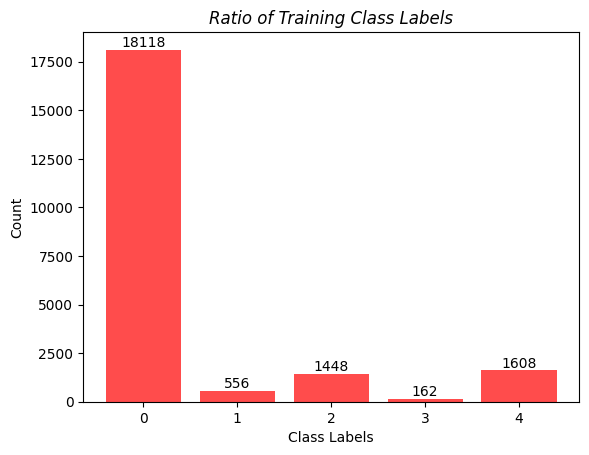
\includegraphics[scale=0.55]{Training Class Label.png} % Replace with your image file name
 \caption{Training Class Label}
 \label{fig:Training Class Label} % Optional: Add a label for the figure
\end{figure}

\section {Data Preprocessing}

\begin{figure}[h]
\centering
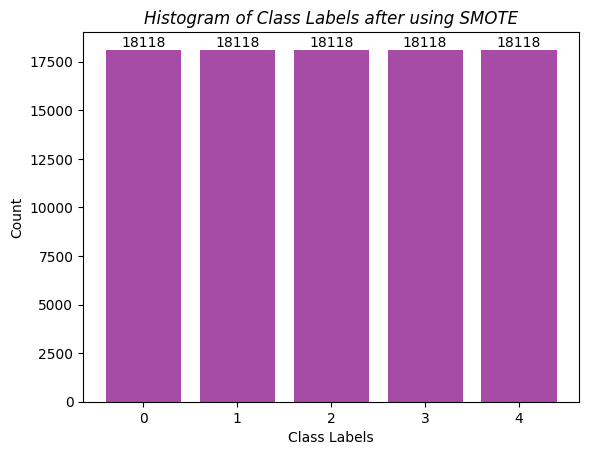
\includegraphics[scale=0.6]{SMOTE.png} % Replace with your image file name
\caption{SMOTE}
\label{fig:SMOTE} % Optional: Add a label for the figure
\end{figure}
To address the problem of imbalanced training data, the SMOTE technique will be used to solve this problem. SMOTE is a synthetic minority over-sampling technique used to address the problem of data imbalance in machine learning. This technique works by synthesizing new data samples for the minority class, which helps to balance the ratio between classes in the dataset. After using SMOTE, the results will be obtained as shown in the diagram below.
\section {Model}
Multi-Layer perceptron (MLP) algorithm is applied with the selected attributes in the input layer and (16, 8) as the hidden layer size. This means that there are two layers of classifiers, including 16 and 8 neurons, for first and second layers, respectively.
\section {Model Evaluation}
\begin{figure}[htp]
\centering
\includegraphics[scale=0.8]{tải xuống (1).png} % Replace with your image file name
\caption{Confusion Matrix}
\label{fig:confusion_matrix} % Optional: Add a label for the figure
\end{figure}

After training the model, we evaluate the model : . First,

\begin{table}[ht]
\centering
\begin{tabular}{|c|cccc|}
\hline
\multicolumn{1}{|c|}{} & Precision & Recall & F1-Score & Support \\ \hline
0 & 0.98 & 0.98 & 0.98 & 72563 \\ \hline
1 & 0.70 & 0.68 & 0.69 & 2293 \\ \hline
2 & 0.88 & 0.91 & 0.89 & 5639 \\ \hline
3 & 0.65 & 0.66 & 0.66 & 634 \\ \hline
4 & 0.96 & 0.96 & 0.96 & 6425 \\ \hline
accuracy &  &  & 0.96 & 87554 \\ \hline
macro avg & 0.84 & 0.84 & 0.84 & 87554 \\ \hline
weighted avg & 0.96 & 0.96 & 0.96 & 87554 \\ \hline
\end{tabular}
\caption{\textbf{Model evaluation for each class}}
\label{tab:my_table} % Optional: Add a label for the table
\end{table}


\section{Conclusion}
Throughout this project, I already implemented the model Multilayer Perceptron,  
\bibliography{my_references}
\end{document}